\subsection{I dont know where to put this yet}

If we start out on anyonic chains, like the $SU(2)_3$ case, this provideds a nice generalization for chains with $C = Rep(SU(2)_k)$ with fusion rules
\[
  j_1 \times j_2 = \sum_{j = \left\vert j_1 - j_2 \right\vert }^{\mathop{\min}(j_1 + j_2, k - j_1 - j_2)} j.
\]
However now, if we approach this in the case of $SU(2)_\infty$ these fusion rules read
\[
  j_1 \times j_2 = \sum_{j = \left\vert j_1 - j_2 \right\vert }^{j_1 + j_2} 
\]
Is this the same as the Q deformations? It is for $q = 1$ and $k=\infty$ but what about the intermediates?

\section{MPO-symmetries}

So im not sure how this works completely but there seems to be way more literature on this than on (globally) symmetric tensors. However this also seems to be connected to anyonic networks. Also to the Category of MPS and MPO?

There is an account of (projective) representation on a peps that act on all levels in \cite{bridgemanEffectiveEdgeStates}. Actually there are more such as \cite[§~IV, Section~2]{cuiperHouchesLectureNotes2026}, \cite{williamsonMatrixProductOperators2016}

Some sources here: On Lattice Models with Module Categories: \cite{eckQuantumLatticeModels2025}, \cite{lootensDualitiesOneDimensionalQuantum2023} \cite{lootensDualitiesOneDimensionalQuantum2024} \cite{lootensEntanglementDensityMatrix2025}. Also chapters IV and V of \cite{cuiperHouchesLectureNotes2026}. On the structure see \cite{liuTradingMathematicalPhysical2025}

I think the original motivation for this is to have the following constraint on MPOs:

\[
  MPO_a \circ MPO_b = \sum_{c}^{} N_{ab}^c MPO_{c} 
\]
which we can obtain by a fusion tensor $X_{ab}^c$ that obeys an intertwining property. 

We immediately obtain our case of global symmetry by encoding
\[
  \rho(g) = \rho_1(g) \otimes \cdots \otimes \rho_n(g)
\]
as a MPO with bond dimension $1$ by setting 
\[
  W^{[a]}_{11,ij} = \rho_a(g)_{ij}
\]

Call $\rho(g) = MPO_g$. Then $\rho(g) \rho(h) = \rho(hg)$ 

If we want $MPO_g MPO_h = MPO_{hg}$ we also have MPO as a unitary representation with bond dimensions $ > 1$. So this generalizes the symmetry approach. 

TODO: check if we can give symmetries such as in the wanniers kramer dual that are given by $Z_i Z_{i+1}$ by not a $Rep(G)$ but instead a $Rep(\mathrm{G} )$ where $\mathrm{G} $ is a groupoid. 

\begin{definition}[2-Category of MPS]
  \label{def:mpsCategory}
  Let $A$ and $B$ be arbitrary MPS with bond collections $d^A, d^B$. Now, define the 1-morphism category $Hom(A \to B)$ where the objects are MPO operators $M$ together with a reduction isometry $Y$.
\end{definition}

I think we may be able to build a nice summary with this diagram:
% https://q.uiver.app/#q=WzAsMTIsWzAsMCwiKEFcXG90aW1lcyBCKVxcb3RpbWVzIEMiXSxbMiwwLCJBIFxcb3RpbWVzIChCIFxcb3RpbWVzIEMpIl0sWzAsMiwiSG9tKChBXFxvdGltZXMgQikgXFxvdGltZXMgQywgRCkiXSxbMiwyLCJIb20oQVxcb3RpbWVzIChCIFxcb3RpbWVzIEMpLCBEKSJdLFswLDUsIlxcZGlzcGxheXN0eWxlXFxiaWdvcGx1c19jIFZee0FCfV9jIFxcb3RpbWVzIFZee2NDfV9EIl0sWzIsNSwiXFxkaXNwbGF5c3R5bGVcXGJpZ29wbHVzX2MgVl57QWN9X0QgXFxvdGltZXMgVl57QkN9X2MiXSxbMSw0LCJcXGNvbmciXSxbMCw2LCJcXHVuZGVyc2V0e1xcYmx1ZXtcXG11IFxcaW4gMSxcXGxkb3RzLCBOXntBQn1fY30gXFxxdWFkIFxcYmx1ZXtcXG51IFxcaW4gMSxcXGxkb3RzLE5ee2NDLER9fX17XFx2ZXJ0IChBLEIpO2M7XFxtdVxccmFuZ2xlIFxcb3RpbWVzIFxcdmVydCBjLEM7IEQ7IFxcbnUgXFxyYW5nbGV9Il0sWzIsNiwiXFxkaXNwbGF5c3R5bGVcXHN1bV97ZixcXGFscGhhLFxcYmV0YX0gW0ZfRF57QUJDfV1feyhjXFxtdVxcbnUpfV57KGZcXGFscGhhXFxiZXRhKX0gXFx2ZXJ0IEEsZjtEO1xcYmV0YVxccmFuZ2xlIFxcb3RpbWVzIFxcdmVydCBCLEM7IGY7IFxcYWxwaGEgXFxyYW5nbGUiXSxbMCw0LCJcXGRpc3BsYXlzdHlsZVxcYmlnb3BsdXNfe2NcXGluIElycihDQVQpfSBIb20oQSBcXG90aW1lcyBCLCBjKSBcXG90aW1lcyBIb20oYyBcXG90aW1lcyBDLCBEKSJdLFsyLDQsIlxcZGlzcGxheXN0eWxlXFxiaWdvcGx1c197ZCBcXGluIElycihcXG1hdGhzZntDYXR9KX0gSG9tKEEgXFxvdGltZXMgZCwgRCkgXFxvdGltZXMgSG9tKEIgXFxvdGltZXMgQywgZCkiXSxbMSw1LCJcXGNvbmciXSxbMCwyLCJIb20oLSxEKSIsMV0sWzEsMywiSG9tKC0sRCkiLDFdLFswLDEsIlxcdW5kZXJzZXR7XFxzaW19e1xcYWxwaGFfe0FCQ319Il0sWzQsNywiXFxpbiIsMyx7InN0eWxlIjp7ImJvZHkiOnsibmFtZSI6Im5vbmUifSwiaGVhZCI6eyJuYW1lIjoibm9uZSJ9fX1dLFs3LDgsIlxcdW5kZXJzZXR7XFxncmVlbntcXHRleHR7Nmotc3ltYm9sc319fXtGXntBQkN9X0R9IiwxLHsic2hvcnRlbiI6eyJzb3VyY2UiOjEwLCJ0YXJnZXQiOjEwfX1dLFsyLDksIlxcdW5kZXJzZXR7XFx0ZXh0e1xcZ3JlZW57c2VtaXNpbXBsaWNpdHl9fX17XFxjb25nfSIsMyx7InN0eWxlIjp7ImJvZHkiOnsibmFtZSI6Im5vbmUifSwiaGVhZCI6eyJuYW1lIjoibm9uZSJ9fX1dLFszLDEwLCJcXHVuZGVyc2V0e1xcdGV4dHtcXGdyZWVue3NlbWlzaW1wbGljaXR5fX19e1xcY29uZ30iLDMseyJvZmZzZXQiOi0yLCJzdHlsZSI6eyJib2R5Ijp7Im5hbWUiOiJub25lIn0sImhlYWQiOnsibmFtZSI6Im5vbmUifX19XSxbOSw0LCI9IiwzLHsic3R5bGUiOnsiYm9keSI6eyJuYW1lIjoibm9uZSJ9LCJoZWFkIjp7Im5hbWUiOiJub25lIn19fV0sWzEwLDUsIj0iLDMseyJzdHlsZSI6eyJib2R5Ijp7Im5hbWUiOiJub25lIn0sImhlYWQiOnsibmFtZSI6Im5vbmUifX19XSxbNSw4LCJcXGluIiwzLHsic3R5bGUiOnsiYm9keSI6eyJuYW1lIjoibm9uZSJ9LCJoZWFkIjp7Im5hbWUiOiJub25lIn19fV0sWzIsMywiXFx1bmRlcnNldHtcXHNpbX17XFxhbHBoYV97QSxCLEN9fSJdLFsyLDMsIlxcc21hbGxcXGdyZWVue1xcdGV4dHthc3NvY2lhdG9yIGluZHVjZXMgaXNvbW9ycGhpbXMgdW5kZXIgeW9uZWRhfX0iLDAseyJvZmZzZXQiOjUsInN0eWxlIjp7ImJvZHkiOnsibmFtZSI6Im5vbmUifSwiaGVhZCI6eyJuYW1lIjoibm9uZSJ9fX1dXQ==
\[\begin{tikzcd}
	{(A\otimes B)\otimes C} && {A \otimes (B \otimes C)} \\
	\\
	{Hom((A\otimes B) \otimes C, D)} && {Hom(A\otimes (B \otimes C), D)} \\
	\\
	{\displaystyle\bigoplus_{c\in Irr(CAT)} Hom(A \otimes B, c) \otimes Hom(c \otimes C, D)} & \cong & {\displaystyle\bigoplus_{d \in Irr(\mathsf{Cat})} Hom(A \otimes d, D) \otimes Hom(B \otimes C, d)} \\
	{\displaystyle\bigoplus_c V^{AB}_c \otimes V^{cC}_D} & \cong & {\displaystyle\bigoplus_c V^{Ac}_D \otimes V^{BC}_c} \\
	{\underset{\blue{\mu \in 1,\ldots, N^{AB}_c} \quad \blue{\nu \in 1,\ldots,N^{cC,D}}}{\vert (A,B);c;\mu\rangle \otimes \vert c,C; D; \nu \rangle}} && {\displaystyle\sum_{f,\alpha,\beta} [F_D^{ABC}]_{(c\mu\nu)}^{(f\alpha\beta)} \vert A,f;D;\beta\rangle \otimes \vert B,C; f; \alpha \rangle} \\
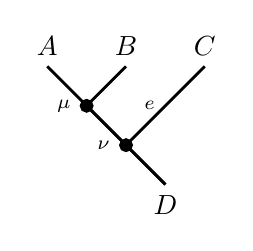
\begin{tikzpicture}[line width=1pt, node distance=1cm]
    % First diagram
    \coordinate (A) at (0,2);
    \coordinate (B) at (1,2);
    \coordinate (C) at (2,2);
    \coordinate (D) at (1.5,0.5);

    \coordinate (V1) at (0.5,1.5);
    \coordinate (V2) at (1.0,1);

    \draw (A) -- (D);
    \draw (B) -- (V1);
    \draw (V1) -- (V2);
    \draw (C) -- (V2);
    \draw (V2) -- (D);

    \filldraw (V1) circle (2pt) node[left=2pt,font=\scriptsize] {$\mu$};
    \filldraw (V2) circle (2pt) node[left=2pt,font=\scriptsize] {$\nu$};

    \node[above] at (A) {$A$};
    \node[above] at (B) {$B$};
    \node[above] at (C) {$C$};
    \node[below] at (D) {$D$};

    \node[left,font=\scriptsize] at (1.5,1.5) {$e$};
\end{tikzpicture}
& =  &
\hspace{-1.8cm}%
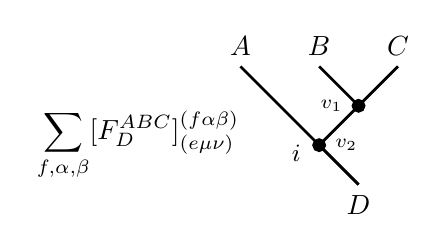
\begin{tikzpicture}[line width=1pt, node distance=1cm, xshift=-2cm]
    \begin{scope}[xshift=-2]
        
    \node at (-1.3,1) 
    {$\displaystyle\sum_{f,\alpha,\beta}
    [F^{ABC}_{D}]_{(e\mu\nu)}^{(f\alpha\beta)}$};

    \coordinate (A) at (0,2);
    \coordinate (B) at (1,2);
    \coordinate (C) at (2,2);
    \coordinate (D) at (1.5,0.5);

    \coordinate (V2) at (1.0,1);
    \coordinate (V1) at (1.5,1.5);

    \draw (A) -- (D);
    \draw (B) -- (V1);
    \draw (V1) -- (V2);
    \draw (C) -- (V1);
    \draw (V2) -- (D);

    \filldraw (V1) circle (2pt) node[left=2pt,font=\scriptsize] {$v_1$};
    \filldraw (V2) circle (2pt) node[right=2pt,font=\scriptsize] {$v_2$};

    \node[above] at (A) {$A$};
    \node[above] at (B) {$B$};
    \node[above] at (C) {$C$};
    \node[below] at (D) {$D$};

    \node[left,font=\small] at (0.9,0.9) {$i$};
    \end{scope}
\end{tikzpicture}
	\arrow["{\underset{\sim}{\alpha_{ABC}}}", from=1-1, to=1-3]
	\arrow["{Hom(-,D)}"{description}, from=1-1, to=3-1]
	\arrow["{Hom(-,D)}"{description}, from=1-3, to=3-3]
	\arrow["{\underset{\sim}{\alpha_{A,B,C}}}", from=3-1, to=3-3]
	\arrow["{\green{\text{associator induces isomorphims under yoneda}}}", shift right=5, draw=none, from=3-1, to=3-3]
	\arrow["{\underset{\text{\green{semisimplicity}}}{\cong}}"{marking, allow upside down}, draw=none, from=3-1, to=5-1]
	\arrow["{\underset{\text{\green{semisimplicity}}}{\cong}}"{marking, allow upside down}, shift left=2, draw=none, from=3-3, to=5-3]
	\arrow["{=}"{marking, allow upside down}, draw=none, from=5-1, to=6-1]
	\arrow["{=}"{marking, allow upside down}, draw=none, from=5-3, to=6-3]
	\arrow["\in"{marking, allow upside down}, draw=none, from=6-1, to=7-1]
	\arrow["\in"{marking, allow upside down}, draw=none, from=6-3, to=7-3]
	\arrow["{\underset{\green{\text{6j-symbols}}}{F^{ABC}_D}}"{description},  from=7-1, to=7-3]
\end{tikzcd}\]
